\newpage
\pagestyle{headings}
\addtocontents{toc}{%
\protect\renewcommand*\protect\cftchappresnum{\appendixname~}}

%\appendix 
%if you have several appendices use the template ubc_2010_spring_doe_jane-appendices.tex
\begin{appendices}
\addappheadtotoc %uses the current page number when it makes the entry in the ToC
\appendixpage %generate a blank Appendix page; 
%note putting Appendix in the same page as the first appendix is not trivial; best found is https://tex.stackexchange.com/questions/374552/appendices-title-on-first-page-of-appendices-and-not-separate-page but the search option of \xpatchcmd does not match since the appendix chapter headers were likely modified from the default by another loaded package

\addtocontents{toc}{
\setlength{\cftbeforechapskip}{\cftbeforesecskip}
\setlength{\cftchapindent}{\cftsecindent}
\protect\renewcommand{\cftchapfont}{\cftsecfont}
\protect\renewcommand{\protect\cftchapdotsep}{\cftsecdotsep}
}

\label{sec:appendices}
\chapter{RFI}
\section{Log-Gamma vs Gaussian Distributions}
\label{sec:gamma_vs_gaussian}
\subsection{Gamma Distribution}
\noindent\textbf{Claim.} A gamma distribution approaches a Gaussian distribution for shape parameter $N \gg 1$.\\

\noindent\textbf{Proof.} Taking the log of a gamma PDF with shape parameter $N$ and scale parameter $\theta$ (written as $f(x)$ instead of $f(x; N, \theta)$ for compactness) gives:
\begin{align}
    \ln f(x) &= \ln \frac{x^{N-1} e^{-x/\theta}}{\theta^N \Gamma(N)} \\[4pt]
     &= (N-1)\ln x - \frac{x}{\theta} - N\ln \theta - \ln \Gamma(N).
\end{align}
The mode can be found by taking the first derivative of the log PDF and setting it to zero:
\begin{align}
    \left.\frac{d}{dx} \ln f(x)\right|_{x=x_0} &= \frac{N-1}{x_0} - \frac{1}{\theta} = 0 \\[4pt]
    \Rightarrow x_0 &= (N-1)\theta \approx N\theta.
\end{align}
The curvature at the mode can be found by taking the second derivative of the log PDF and evaluating it at the mode:
\begin{align}
    \left.\frac{d^2}{dx^2} \ln f(x)\right|_{x=x_0} &= -\frac{N-1}{x_0^2} \\[4pt]
    &=-\frac{1}{(N-1)\theta^2} \approx -\frac{1}{N\theta^2}.
\end{align}
Taking a Taylor expansion of the log PDF around the mode $x_0$, noting that the derivative of $\ln f(x)$ vanishes at $x = x_0$ since $x_0$ is the mode, gives:
\begin{align}
    \ln f(x) &= \ln f(x_0) + \frac{1}{2} \left.\frac{d^2}{dx^2} \ln f(x)\right|_{x=x_0} (x - x_0)^2 + \dots \\[4pt]
    &\approx \ln f(x_0) - \frac{(x - x_0)^2}{2N\theta^2}.
\end{align}
Exponentiating,
\begin{align}
    f(x) &\approx C \exp\left(-\frac{(x - x_0)^2}{2N\theta^2}\right) \\[4pt]
    &\approx C \exp\left(-\frac{(x - N\theta)^2}{2N\theta^2}\right).
\end{align}

Consider a Gaussian distribution with mean $N\theta$ and variance $N\theta^2$:
\begin{align}
    g(x; N\theta, N\theta^2) &= \frac{1}{\sqrt{2\pi N\theta^2}} \exp\left(-\frac{(x - N\theta)^2}{2N\theta^2}\right) \\[4pt]
    &= C \exp\left(-\frac{(x - N\theta)^2}{2N\theta^2}\right).
\end{align}
This shows that the PDF of the gamma distribution approaches the PDF of the Gaussian distribution up to a constant $C$ as $N$ becomes large, so that $N-1 \approx N$. It can be shown that the constant $C$ is equal to $1/\sqrt{2\pi N\theta^2}$ by normalizing the gamma distribution and using Stirling's approximation for the gamma function. However, the normalizing constant does not impact the kurtosis, so the full derivation of it is omitted.

\subsection{Log-Gamma Distribution}
\noindent\textbf{Claim.} The log of a gamma distribution approaches a Gaussian distribution for shape parameter $N \gg 1$.\\

\noindent\textbf{Proof.} Let $W$ be a log-gamma random variable defined as $W = \ln X$ where $X \sim \text{Gamma}(N, \theta)$. By a change of variables with
$x = e^{w}$ and $dx = e^{w}\,dw$, the PDF of $W$ is
\begin{align}
    f_W(w) &= f_X(e^{w})\,e^{w}
        = \frac{(e^{w})^{N-1} e^{-e^{w}/\theta}}{\theta^N \Gamma(N)}\,e^{w} \\[4pt]
    &= \frac{e^{Nw}\, e^{-e^{w}/\theta}}{\theta^N \Gamma(N)}.
\end{align}
The log PDF is
\begin{equation}
    \ln f_W(w) = Nw - \frac{e^{w}}{\theta} - N\ln\theta - \ln\Gamma(N).
\end{equation}
Applying the same procedure as above, the mode and curvature are obtained from the first two derivatives:
\begin{align}
    \left.\frac{d}{dw}\ln f_W(w)\right|_{w=w_0} &= N - \frac{e^{w_0}}{\theta} = 0
        \;\Rightarrow\; w_0 = \ln(N\theta), \\[4pt]
    \left.\frac{d^2}{dw^2}\ln f_W(w)\right|_{w=w_0} &= -\frac{e^{w_0}}{\theta} = -N.
\end{align}
Taking the Taylor expansion about the mode, where again the first derivative term is zero, gives:
\begin{align}
    \ln f_W(w) &= \ln f_W(w_0) + \frac{1}{2}\left.\frac{d^2}{dw^2}\ln f_W(w)\right|_{w=w_0} (w - w_0)^2 + \dots \\[4pt]
    &\approx \ln f_W(w_0) - \frac{N}{2}(w - w_0)^2.
\end{align}
After exponentiating, the approximate form of the log-gamma PDF is
\begin{equation}
    f_W(w; N, \theta) \approx C \exp\left(-\frac{N(w - w_0)^2}{2}\right).
\end{equation}
This shows that the PDF of a log-gamma random variable $W = \ln X$ is approximately Gaussian  to second order, with mean $w_0 = \ln(N\theta)$ and variance $1/N$. 

\section{Spectral Kurtosis Pair Plot}
\label{sec:spectral_kurtosis_pair_plot}

\begin{figure}[H]
    \centering
    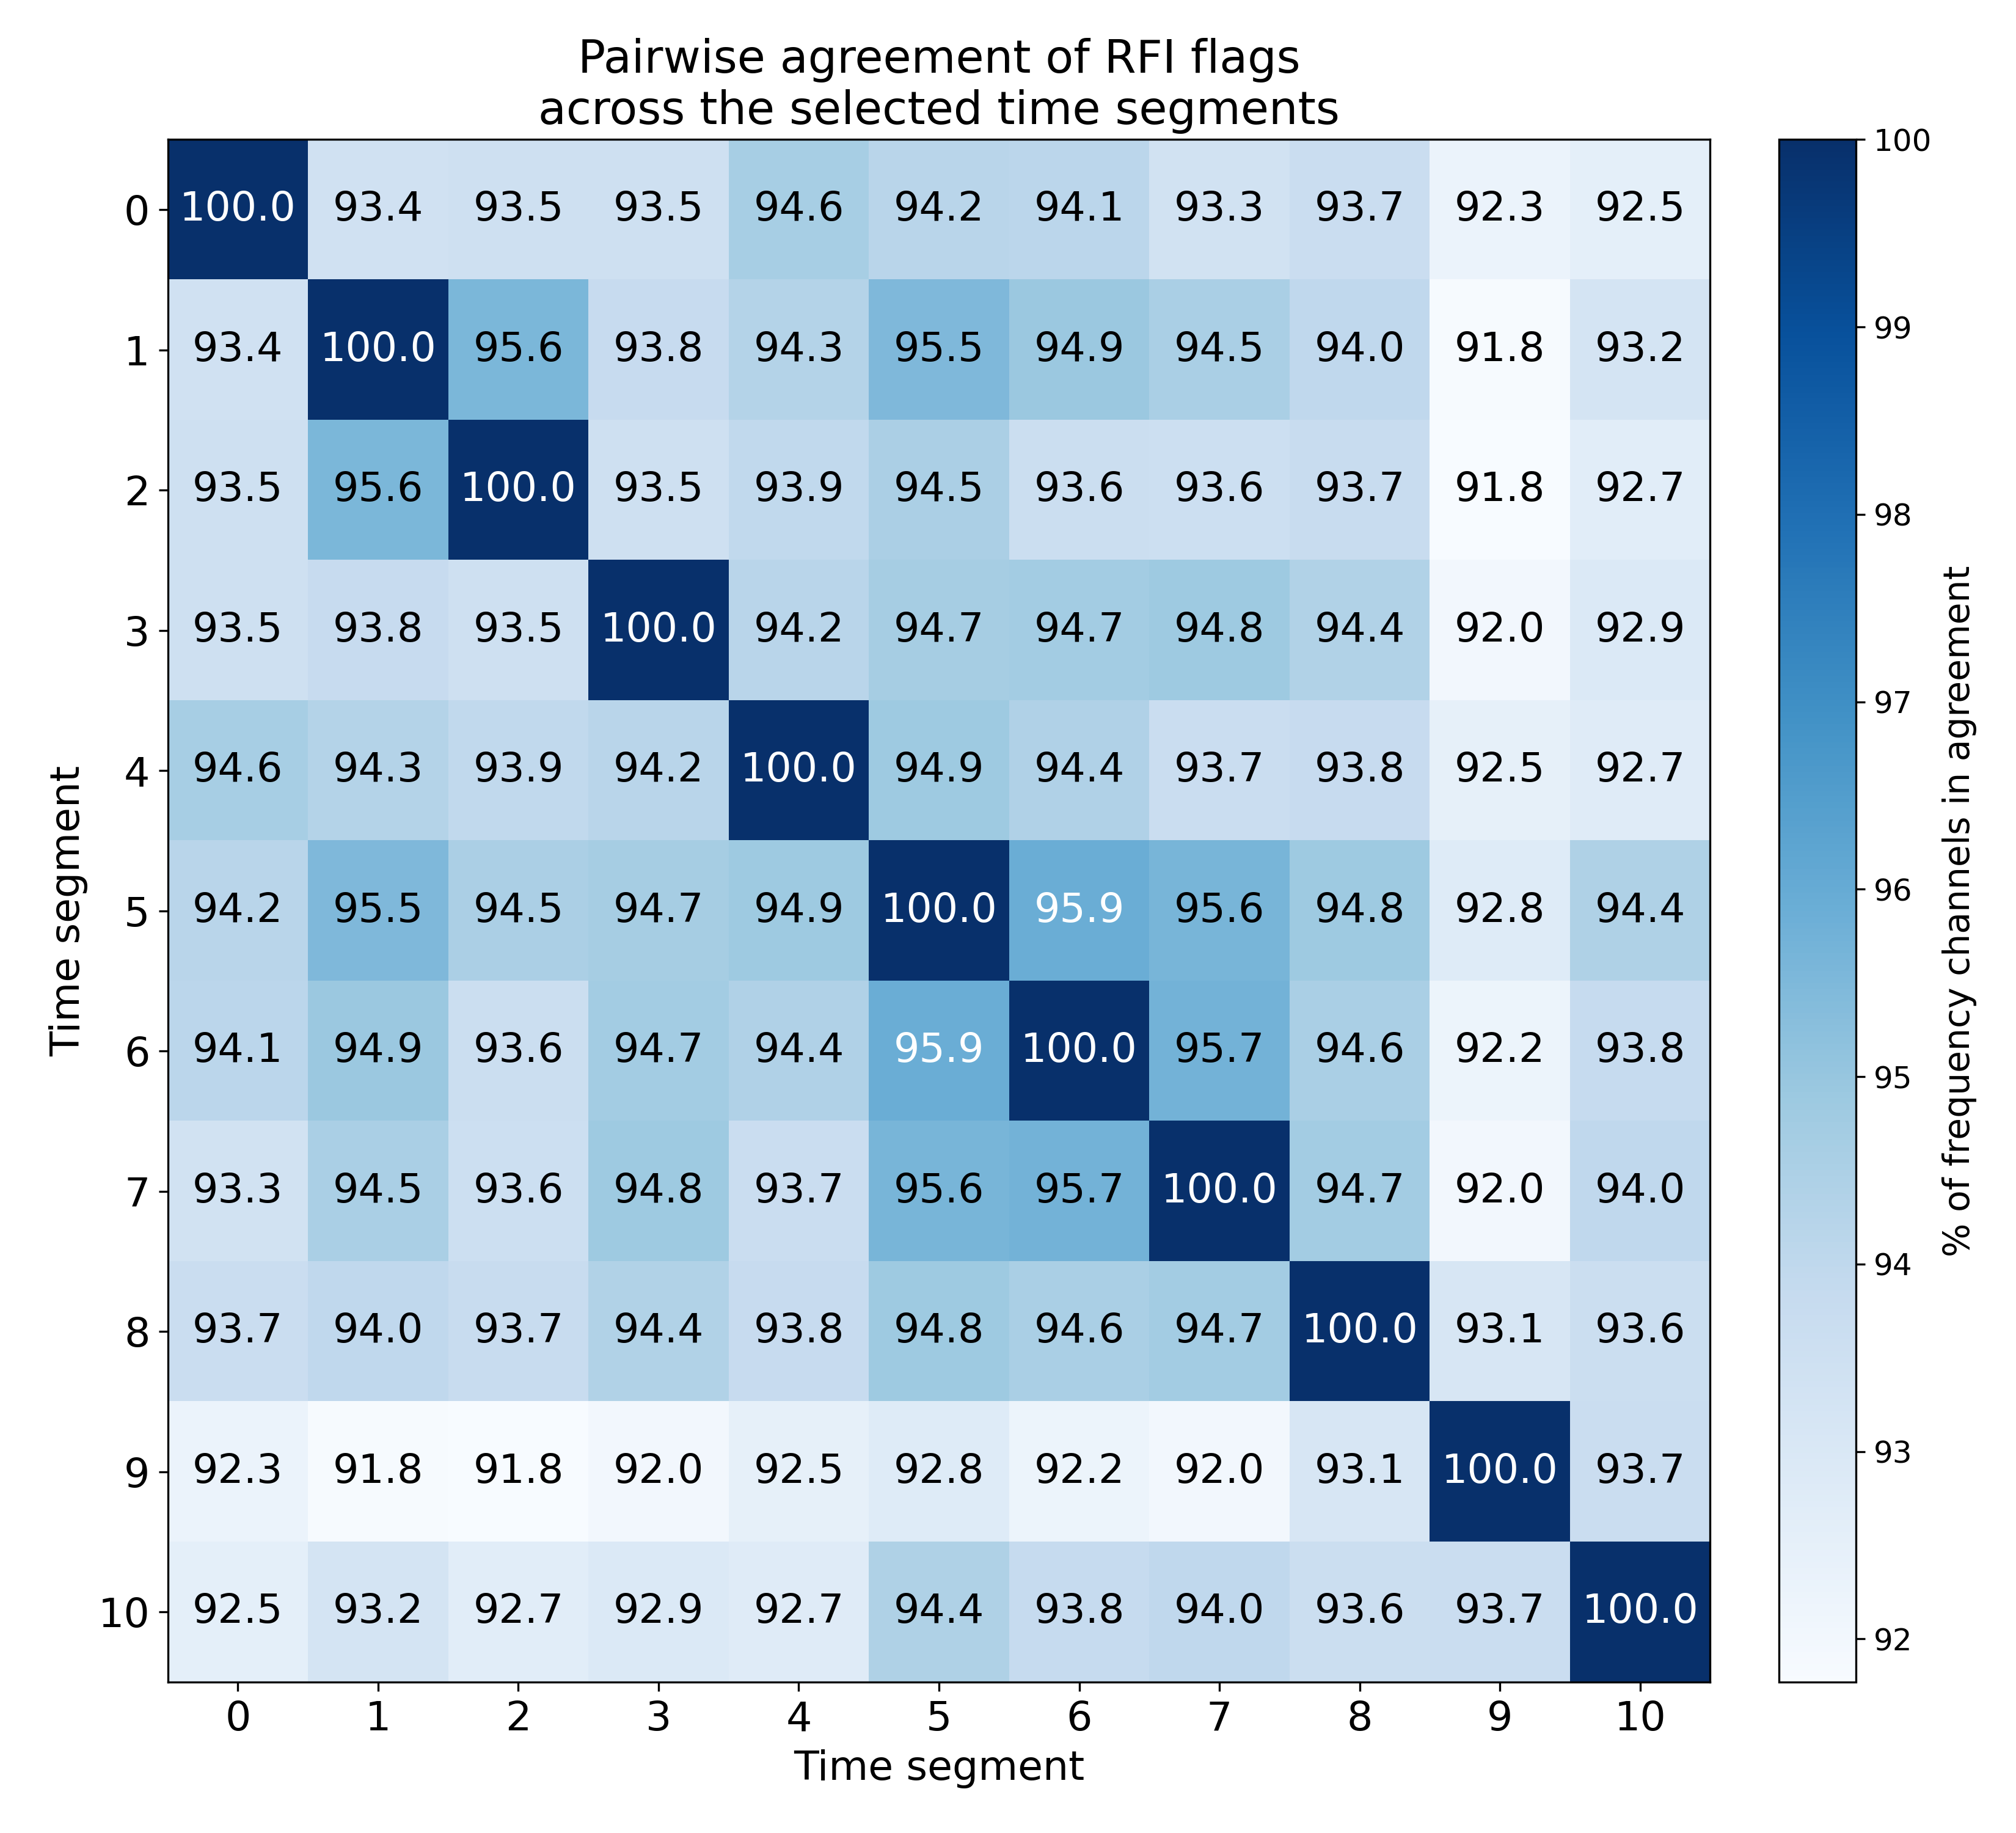
\includegraphics[width=1\linewidth]{thesis/plots/rfi/rfi_flag_agreement.png}
    \caption[Pair plot of RFI label agreement]{Pair plot of agreement between RFI labels for each of the 11 time segments showing the extent of agreement between each pair of segments.}
    \label{fig:spectral_kurtosis_pair_plot}
\end{figure}

\section{Alternative RFI Thresholds}
\label{sec:alternative_rfi_thresholds}

Two subjective design decisions were made in the RFI analysis of section~\ref{sec:excess_kurtosis_rfi_detection}. The first was to use RFI thresholds of [0.1\%, 99.9\%] on calibrated spectral kurtosis. These thresholds were chosen as deliberately wide to reduce false positives (clean spectrum labelled RFI); however, they also increase false negatives (RFI spectrum labelled clean). Secondly, while aggregating the 11 independent time segments, we assumed that if at least 6 of the 11 segments are clean (`50\%') we consider the frequency clean; alternative approaches are to require that at least one of the segments be clean (`any') or that all segments be clean (`all'), representing more permissive and more strict approaches respectively. The results of these alternative approaches are shown in table \ref{tbl:rrl_clean_counts}.\\

\begin{table}[h!]
\centering
\caption{Number of detectable hydrogen RRLs per frequency region, by cross-segment aggregation method (any/50\%/all) and spectral kurtosis threshold (0.1\%, 0.5\%, 1\%).}
\label{tbl:rrl_clean_counts}
\begin{tabular}{lccccccccc}
\toprule
\textbf{Aggregation:} & \multicolumn{3}{c}{\textbf{any}} & \multicolumn{3}{c}{\textbf{50\%}} & \multicolumn{3}{c}{\textbf{all}} \\
\cmidrule(lr){2-4} \cmidrule(lr){5-7} \cmidrule(lr){8-10}
\textbf{SK Threshold:} & 0.1\% & 0.5\% & 1\% & 0.1\% & 0.5\% & 1\% & 0.1\% & 0.5\% & 1\% \\
\midrule
Low frequency  & 32 & 32 & 32 & 29 & 29 & 29 & 0 & 0 & 0 \\
Mid frequency  & 26 & 26 & 26 & 23 & 23 & 23 & 1 & 0 & 0 \\
High frequency & 32 & 32 & 31 & 27 & 26 & 25 & 0 & 0 & 0 \\
\midrule
\textbf{Total} & 90 & 90 & 89 & 79 & 78 & 77 & 1 & 0 & 0 \\
\bottomrule
\end{tabular}
\end{table}

The results show that the choice of SK threshold has a minimal impact on total visible lines, impacting between just one or two lines. Meanwhile the aggregation method changes results significantly from 90 visible lines to just 1.

To understand the sensitivity to aggregation, we can imagine a spectrum that is completely RFI free. If we choose a 0.1\% SK threshold then we expect a 0.2\% false positive rate per channel per time segment (given that its a two sided test). Choosing the `any' aggregation method, the channel is clean if at least one time segment is not a false positive, which  has probability \(1 -0.002^{11}\approx1\). The `50\%' aggregation will be clean if at least 6 of 11 channels are not false positives, using the binomial distribution this has probability \(P(X\ge 6) = \sum_{k=6}^{11}{11 \choose k}0.998^k\cdot0.002^{11-k}\approx1\). For both previous cases the probability of aggregating a false positive is essentially zero. Meanwhile, for the `all' aggregation, the channel is clean when all time segments are clean which has probability \(0.998^{11} = 0.978\), so the probability of a false positive per channel is 2.2\%. We consider an RRL to be detectable by taking the Gaussian weighted average across a 400 km s$^{-1}$ profile, which comprises 120 channels at 300~MHz or 592 channels at 1500~MHz. Given a 2.2\% false positive rate, the probability that one or more of the 120 channels are false positive is \(1-0.978^{120}=0.93\), meaning that the line is likely to be characterized as undetectable based on false positives alone, explaining why the `all' aggregation shows no detectable lines.

Since the probability of aggregating a false positive in both the `any' aggregation and `50\%' aggregation is extremely low, the differences we observe in detectable lines between them is likely the result of genuine intermittent RFI being detected and not just statistical noise.



\chapter{Extension CHORD}
\section{Additional Extension CHORD Plots}
\label{sec:ext_chord_appendix}

\subsection{Pairwise comparisons}

Pairwise comparisons were performed by looking at natural weighting, robust weighting with R=0, and uniform weighting for each permutation of extension CHORD locations. The combination B + D emerges as the best candidate in every weighting scheme. A combined metric of resolution times noise factor which attempts to balance the trade-off between resolution and sensitivity also shows that B + D is the best candidate across all weighting schemes. The pairwise comparisons are shown in Figure \ref{fig:pairwise_comparisons}.

\begin{figure}[h]
    \centering
    \begin{subfigure}[b]{\textwidth}
        \centering
        
\includegraphics[width=\textwidth]{pairplot_resolution_noise_natural.png}
    \end{subfigure}
    \begin{subfigure}[b]{\textwidth}
        \centering
        
\includegraphics[width=\textwidth]{pairplot_resolution_noise_briggs0.png}
    \end{subfigure}
    \begin{subfigure}[b]{\textwidth}
        \centering
        
\includegraphics[width=\textwidth]{pairplot_resolution_noise_uniform.png}
    \end{subfigure}
    \caption{Resolution and Resolution x Noise Factor pairwise comparisons for natural, robust (R=0), and uniform weighting schemes. B + D emerges as the best candidate in every comparison method.}
    \label{fig:pairwise_comparisons}
\end{figure}

\subsection{UV coverage of B + D}

A plot of the UV coverage of B, D, and B + D is shown in Figure \ref{fig:uv_coverage_B_D} which shows the complementary nature of the two locations and that the combined UV coverage plot is well-filled.
\begin{figure}[h]
    \centering
    
\includegraphics[width=\textwidth]{uv_coverage_B_D_BD.png}
    \caption{UV coverage of B, D and B + D configuration showing the complementary nature of the two locations.}
    \label{fig:uv_coverage_B_D}
\end{figure}


\chapter{Appendix C: SIGGMA Results}
\section{Complete SIGGMA tables}
\label{sec:siggma_appendix}

\subsection{SIGGMA HII Regions}
A complete set of the reported HII regions produced by SIGGMA which are also visible to CHORD..

\begin{table}[H]
    \centering
    \begin{tabular}{l c c c c c}
        \toprule
        Order & Name & Peak [mK] & FWHM [km/s] & S/N & Type \\
        \midrule
        1 & G063.164+00.449 & $694.5 \pm 40.6$ & $16.5 \pm 1.1$ & 16.9 & Known \\
        2 & G061.473+00.094 & $348.6 \pm 26.9$ & $30.1 \pm 2.7$ & 12.8 & Known \\
        3 & G059.796+00.241 & $124.5 \pm 11.4$ & $33.2 \pm 3.5$ & 10.7 & Known \\
        4 & G059.321-00.223 & $124.1 \pm 4.3$ & $23.7 \pm 1.0$ & 28.5 & Known \\
        5 & G062.921+00.079 & $107.2 \pm 4.0$ & $23.8 \pm 1.0$ & 26.7 & Known \\
        6 & G061.292-00.331 & $83.8 \pm 17.2$ & $41.2 \pm 9.8$ & 5.0 & Known \\
        7 & G056.725-00.179 & $78.1 \pm 6.5$ & $75.8 \pm 7.3$ & 11.8 & Candidate \\
        8 & G055.567+00.701 & $75.3 \pm 2.8$ & $19.1 \pm 0.8$ & 26.6 & Candidate \\
        9 & G057.541-00.279 & $66.6 \pm 7.3$ & $26.6 \pm 3.4$ & 12.9 & Known \\
        10 & G063.050-00.124 & $65.3 \pm 2.5$ & $24.9 \pm 1.1$ & 26.0 & Candidate \\
        11 & G060.881-00.135 & $57.5 \pm 8.1$ & $28.2 \pm 6.0$ & 12.7 & Known \\
        12 & G057.624+00.410 b & $54.6 \pm 5.8$ & $74.4 \pm 12.1$ & 21.8 & Candidate \\
        13 & G057.545-00.275 & $52.4 \pm 7.5$ & $16.1 \pm 3.8$ & 7.5 & Known \\
        14 & G056.083-00.176 & $51.3 \pm 6.3$ & $15.6 \pm 2.2$ & 8.0 & Known \\
        15 & G057.624+00.410 b & $50.7 \pm 11.3$ & $14.5 \pm 4.0$ & 9.0 & Candidate \\
        16 & G064.130-00.475 & $45.4 \pm 3.0$ & $27.9 \pm 2.1$ & 14.9 & Known \\
        17 & G063.052-00.332 & $41.5 \pm 3.6$ & $43.5 \pm 4.4$ & 11.5 & Known \\
        18 & G061.467+00.380 & $38.9 \pm 3.0$ & $20.5 \pm 1.8$ & 12.9 & Known \\
        19 & G067.816+00.511 & $27.2 \pm 4.9$ & $19.1 \pm 4.0$ & 5.4 & Candidate \\
        20 & G061.144-00.891 & $25.1 \pm 4.6$ & $18.4 \pm 3.9$ & 5.4 & Candidate \\
        21 & G059.600+00.316 & $23.4 \pm 3.5$ & $28.6 \pm 5.0$ & 6.6 & Known \\
        22 & G057.715+00.173 & $19.5 \pm 2.6$ & $33.8 \pm 7.2$ & 13.3 & Candidate \\
        23 & G061.053-00.825 b & $19.1 \pm 3.2$ & $47.9 \pm 9.3$ & 5.9 & Candidate \\
        24 & G057.715+00.173 & $18.0 \pm 2.9$ & $22.7 \pm 4.9$ & 10.0 & Candidate \\
        25 & G057.715+00.173 & $17.1 \pm 1.7$ & $68.7 \pm 11.3$ & 16.6 & Candidate \\
        26 & G062.142-00.144 & $16.8 \pm 2.6$ & $63.9 \pm 11.7$ & 6.2 & Candidate \\
        \bottomrule
    \end{tabular}
    \caption{Set of SIGGMA HII regions and candidate HII regions visible to CHORD.}
    \label{tab:siggma_candidates}
\end{table}


\subsection{SIGGMA Stacked SNR Predictions}

A complete set of the predicted SNR levels which CHORD can achieve on the HII regions reported by SIGGMA. Using a common frequency resolution of \( 5 \kHz \) and each line's native angular resolution.

\begin{table}[H]
    \centering
    \begin{tabular}{l c c c c}
        \toprule
        Order & Name & SNR top 1 & SNR top 15 & SNR top 60 \\
        \midrule
        1 & G063.164+00.449 & $23.55 \pm 1.38$ & $90.98 \pm 5.32$ & $171.54 \pm 10.03$ \\
        2 & G061.473+00.094 & $9.72 \pm 0.75$ & $37.47 \pm 2.89$ & $70.73 \pm 5.46$ \\
        3 & G059.796+00.241 & $3.71 \pm 0.34$ & $14.26 \pm 1.31$ & $26.71 \pm 2.45$ \\
        4 & G059.321-00.223 & $3.69 \pm 0.13$ & $14.21 \pm 0.49$ & $26.79 \pm 0.93$ \\
        5 & G062.921+00.079 & $3.73 \pm 0.14$ & $14.42 \pm 0.54$ & $27.14 \pm 1.01$ \\
        6 & G061.292-00.331 & $2.75 \pm 0.56$ & $10.60 \pm 2.18$ & $19.94 \pm 4.09$ \\
        7 & G056.725-00.179 & $2.64 \pm 0.22$ & $10.18 \pm 0.85$ & $19.07 \pm 1.59$ \\
        8 & G055.567+00.701 & $2.38 \pm 0.09$ & $9.15 \pm 0.34$ & $17.12 \pm 0.64$ \\
        9 & G057.541-00.279 & $2.22 \pm 0.24$ & $8.55 \pm 0.94$ & $16.02 \pm 1.76$ \\
        10 & G063.050-00.124 & $2.33 \pm 0.09$ & $8.99 \pm 0.34$ & $16.90 \pm 0.65$ \\
        11 & G060.881-00.135 & $1.78 \pm 0.25$ & $6.87 \pm 0.97$ & $12.92 \pm 1.82$ \\
        12 & G057.624+00.410 b & $1.75 \pm 0.19$ & $6.72 \pm 0.71$ & $12.59 \pm 1.34$ \\
        13 & G057.545-00.275 & $1.75 \pm 0.25$ & $6.72 \pm 0.96$ & $12.59 \pm 1.80$ \\
        14 & G056.083-00.176 & $1.70 \pm 0.21$ & $6.54 \pm 0.80$ & $12.28 \pm 1.51$ \\
        15 & G057.624+00.410 b & $1.62 \pm 0.36$ & $6.24 \pm 1.39$ & $11.69 \pm 2.60$ \\
        16 & G064.130-00.475 & $1.71 \pm 0.11$ & $6.60 \pm 0.44$ & $12.38 \pm 0.82$ \\
        17 & G063.052-00.332 & $1.51 \pm 0.13$ & $5.83 \pm 0.51$ & $10.95 \pm 0.95$ \\
        18 & G061.467+00.380 & $1.26 \pm 0.10$ & $4.87 \pm 0.38$ & $9.16 \pm 0.71$ \\
        19 & G067.816+00.511 & $1.04 \pm 0.19$ & $4.00 \pm 0.72$ & $7.50 \pm 1.35$ \\
        20 & G061.144-00.891 & $0.87 \pm 0.16$ & $3.36 \pm 0.62$ & $6.32 \pm 1.16$ \\
        21 & G059.600+00.316 & $0.75 \pm 0.11$ & $2.88 \pm 0.43$ & $5.41 \pm 0.81$ \\
        22 & G057.715+00.173 & $0.62 \pm 0.08$ & $2.40 \pm 0.32$ & $4.48 \pm 0.60$ \\
        23 & G061.053-00.825 b & $0.66 \pm 0.11$ & $2.56 \pm 0.43$ & $4.80 \pm 0.80$ \\
        24 & G057.715+00.173 & $0.58 \pm 0.09$ & $2.21 \pm 0.36$ & $4.14 \pm 0.67$ \\
        25 & G057.715+00.173 & $0.55 \pm 0.05$ & $2.10 \pm 0.21$ & $3.93 \pm 0.39$ \\
        26 & G062.142-00.144 & $0.61 \pm 0.09$ & $2.37 \pm 0.37$ & $4.45 \pm 0.69$ \\
        \bottomrule
    \end{tabular}
    \caption{SNR for CHORD observations of SIGGMA HII regions using one observing day, showing the SNR for the top 1, 15 and 60 stacked lines.}
    \label{tab:siggma_stacked_snr}
\end{table}


\subsection{SIGGMA Stacked SNR Predictions with Smoothing}

A complete set of the predicted SNR levels which CHORD can achieve on the HII regions reported by SIGGMA, after smoothing to a common velocity resolution of \( 5 \kms \) and a common angular resolution as reported in the table header.

\begin{table}[H]
    \centering
    \begin{tabular}{l c c c c c}
        \toprule
        Order & Name & SNR $5'$ & SNR $6'$ & SNR $8'$ & SNR $12'$ \\
        \midrule
        1 & G063.164+00.449 & $85.04 \pm 4.97$ & $130.52 \pm 7.63$ & $222.38 \pm 13.00$ & $368.23 \pm 21.53$ \\
        2 & G061.473+00.094 & $41.86 \pm 3.23$ & $63.49 \pm 4.90$ & $105.47 \pm 8.14$ & $171.58 \pm 13.24$ \\
        3 & G059.796+00.241 & $14.70 \pm 1.35$ & $22.45 \pm 2.06$ & $37.98 \pm 3.48$ & $62.37 \pm 5.71$ \\
        4 & G059.321-00.223 & $14.70 \pm 0.51$ & $22.44 \pm 0.78$ & $37.79 \pm 1.31$ & $61.96 \pm 2.15$ \\
        5 & G062.921+00.079 & $13.05 \pm 0.49$ & $20.08 \pm 0.75$ & $34.37 \pm 1.28$ & $57.11 \pm 2.13$ \\
        6 & G061.292-00.331 & $10.04 \pm 2.06$ & $15.43 \pm 3.17$ & $26.35 \pm 5.41$ & $43.60 \pm 8.95$ \\
        7 & G056.725-00.179 & $9.24 \pm 0.77$ & $14.21 \pm 1.18$ & $24.57 \pm 2.04$ & $40.95 \pm 3.41$ \\
        8 & G055.567+00.701 & $8.91 \pm 0.33$ & $13.70 \pm 0.51$ & $23.42 \pm 0.87$ & $38.68 \pm 1.44$ \\
        9 & G057.541-00.279 & $7.92 \pm 0.87$ & $12.18 \pm 1.34$ & $20.99 \pm 2.30$ & $34.89 \pm 3.82$ \\
        10 & G063.050-00.124 & $7.98 \pm 0.31$ & $12.29 \pm 0.47$ & $21.11 \pm 0.81$ & $35.15 \pm 1.35$ \\
        11 & G060.881-00.135 & $6.84 \pm 0.96$ & $10.47 \pm 1.47$ & $17.74 \pm 2.50$ & $29.20 \pm 4.11$ \\
        12 & G057.624+00.410 b & $6.48 \pm 0.69$ & $9.96 \pm 1.06$ & $17.05 \pm 1.81$ & $28.21 \pm 3.00$ \\
        13 & G057.545-00.275 & $6.22 \pm 0.89$ & $9.57 \pm 1.37$ & $16.50 \pm 2.36$ & $27.43 \pm 3.93$ \\
        14 & G056.083-00.176 & $6.09 \pm 0.75$ & $9.36 \pm 1.15$ & $16.07 \pm 1.97$ & $26.68 \pm 3.28$ \\
        15 & G057.624+00.410 b & $6.02 \pm 1.34$ & $9.25 \pm 2.06$ & $15.83 \pm 3.53$ & $26.19 \pm 5.84$ \\
        16 & G064.130-00.475 & $5.62 \pm 0.37$ & $8.69 \pm 0.57$ & $15.03 \pm 0.99$ & $25.15 \pm 1.66$ \\
        17 & G063.052-00.332 & $5.07 \pm 0.44$ & $7.82 \pm 0.68$ & $13.48 \pm 1.17$ & $22.51 \pm 1.95$ \\
        18 & G061.467+00.380 & $4.66 \pm 0.36$ & $7.16 \pm 0.55$ & $12.17 \pm 0.94$ & $20.10 \pm 1.55$ \\
        19 & G067.816+00.511 & $3.40 \pm 0.61$ & $5.27 \pm 0.95$ & $9.12 \pm 1.64$ & $15.26 \pm 2.75$ \\
        20 & G061.144-00.891 & $3.05 \pm 0.56$ & $4.70 \pm 0.86$ & $8.09 \pm 1.48$ & $13.45 \pm 2.46$ \\
        21 & G059.600+00.316 & $2.76 \pm 0.41$ & $4.23 \pm 0.63$ & $7.23 \pm 1.08$ & $11.95 \pm 1.79$ \\
        22 & G057.715+00.173 & $2.31 \pm 0.31$ & $3.54 \pm 0.47$ & $6.07 \pm 0.81$ & $10.05 \pm 1.34$ \\
        23 & G061.053-00.825 b & $2.31 \pm 0.39$ & $3.57 \pm 0.60$ & $6.14 \pm 1.03$ & $10.21 \pm 1.71$ \\
        24 & G057.715+00.173 & $2.13 \pm 0.34$ & $3.27 \pm 0.53$ & $5.60 \pm 0.90$ & $9.27 \pm 1.49$ \\
        25 & G057.715+00.173 & $2.02 \pm 0.20$ & $3.11 \pm 0.31$ & $5.32 \pm 0.53$ & $8.81 \pm 0.88$ \\
        26 & G062.142-00.144 & $2.03 \pm 0.31$ & $3.13 \pm 0.49$ & $5.42 \pm 0.84$ & $9.07 \pm 1.40$ \\
        \bottomrule
    \end{tabular}
    \caption{SNR for CHORD observations of SIGGMA HII regions with a smoothed angular resolution of 5, 6, 8 and 12 arcminutes.}
    \label{tab:siggma_stacked_snr}
\end{table}


\end{appendices}